\documentclass[tikz,border=2pt]{standalone}
\usetikzlibrary{calc}
\usetikzlibrary{intersections}
\usetikzlibrary{patterns}
\usepackage{bm}

\begin{document}

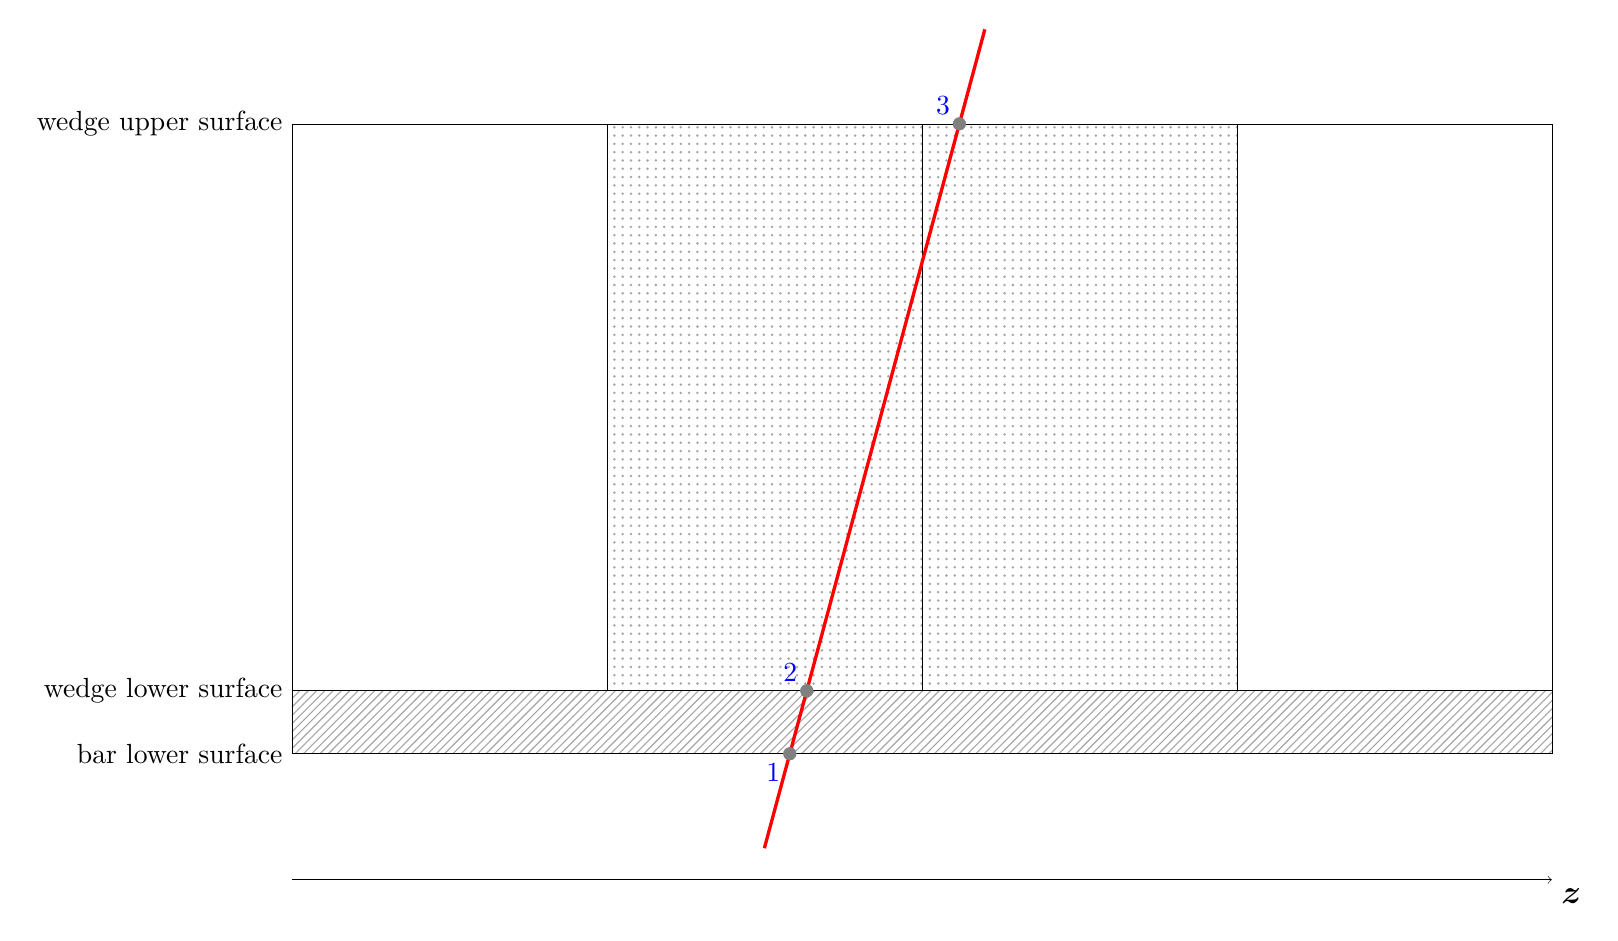
\begin{tikzpicture}[scale=4, very thin]
    
    % draw a bar
    \filldraw [pattern color=gray!70, draw=black, pattern=north east lines] (0,0) rectangle (4,0.2);
    % wedges
    \draw (0,0.2) rectangle (1,2);
    \filldraw [pattern color=gray!70, draw=black, pattern=dots] (1,0.2) rectangle (2,2);
    \filldraw [pattern color=gray!70, draw=black, pattern=dots] (2,0.2) rectangle (3,2);
    \draw (3,0.2) rectangle (4,2);

    % draw a track
    \coordinate (A) at (1.5,-0.3);
    \coordinate (B) at (2.2,2.3);
    \draw[very thick, red, name path=track] (A)  -- (B);

    % define path
    \path[name path=upperWedge] (0,2) -- (3,2);
    \path[name path=lowerWedge] (0,0.2) -- (3,0.2);
    \path[name path=lowerBar] (0,0) -- (3,0);

    % get intersections
    \path[name intersections={of=lowerBar and track, by=I1}];
    \path[name intersections={of=lowerWedge and track, by=I2}];
    \path[name intersections={of=upperWedge and track, by=I3}];

    % display intersection point
    \filldraw[gray] (I1) circle [radius=0.02];
    \node [below left, blue] at (I1) {$1$};

    \filldraw[gray] (I2) circle [radius=0.02];
    \node [above left, blue] at (I2) {$2$};

    \filldraw[gray] (I3) circle [radius=0.02];
    \node [above left, blue] at (I3) {$3$};

    % display z axis
    %\draw[->] (0,0 |- A) -- (4,0 |- A);
    %\node [below right] at (4,0 |- A) {$z$};
    \draw[->] (0,-0.4) -- (4,-0.4);
    \node [below right] at (4,-0.4) {\large $\bm{z}$};

    % add text
    \node[left] at (0,0) {bar lower surface};
    \node[left] at (0,0.2) {wedge lower surface};
    \node[left] at (0,2) {wedge upper surface};
    
    

\end{tikzpicture}


\end{document}